%
% Copyright 2018 Joel Feldman, Andrew Rechnitzer and Elyse Yeager.
% This work is licensed under a Creative Commons Attribution-NonCommercial-ShareAlike 4.0 International License.
% https://creativecommons.org/licenses/by-nc-sa/4.0/
%

\questionheader{ex:s3.4.7}


%%%%%%%%%%%%%%%%%%
\subsection*{\Conceptual}
%%%%%%%%%%%%%%%%%%

\begin{question}
Let $f(x)=7x^2-3x+4$.
Suppose we measure $x$ to be $x_0 = 2$
        but that the real value of $x$ is $x_0+\Delta x$. Suppose further that
        the error in our measurement is $\Delta x = 1$.
Let $\Delta y$ be the change in $f(x)$ corresponding to a change of $\Delta x $ in $x_0$. That is,
$\Delta y = f\left(x_0+\Delta x\right)-f(x_0)$.

True or false: $\Delta y = f'(2)(1)=25$
\end{question}
\begin{hint}
Is the linear approximation exact, or approximate?
\end{hint}
\begin{answer} False.
\end{answer}
\begin{solution}
False. The linear approximation is an \emph{approximation}. It tells us
\[\Delta  y \approx  f'(x_0)\Delta x=f'(2)(1)=25\]
However, from our definition of $\Delta y$,
\[\Delta y = f(x_0+\Delta x)-f(x_0)=f(2+1)-f(2)=58-26=32\]

Remark: this is to emphasize that the calculations in this subsection are \emph{estimations} of error bounds, rather than actual error bounds. All we can say is that we \emph{estimate} the error will be no more than some number--we don't guarantee it.

In the next subsection, we will introduce an error bound that is guaranteed to be accurate. It is usually harder to calculate than the estimations in this section.
\end{solution}





\begin{question}
Suppose the exact amount you are supposed to tip is \$5.83, but you approximate and tip \$6. What is the absolute error in your tip? What is the percent error in your tip?
\end{question}
\begin{hint}
When an exact value $Q_0$ is measured as $Q_0+\Delta Q$,
Definition~\ref*{def:APPrelError}
%3.4.25
gives us the absolute error as $|\Delta Q|$, and the percentage error as $100\dfrac{|\Delta Q|}{Q_0}$.
\end{hint}
\begin{answer}
Absolute error: 0.17; percentage error: 2.92\%
\end{answer}
\begin{solution}
When an exact value $Q_0$ is measured as $Q_0+\Delta Q$,
Definition~\ref*{def:APPrelError}
%3.4.25
gives us the absolute error as $|\Delta Q|$, and the percentage error as $100\dfrac{|\Delta Q|}{Q_0}$.

In our situation, $Q_0=5.83$ and $Q_0+\Delta Q = 6$, so $\Delta Q = 0.17$. So, the absolute error is $0.17$, and the percentage error is
\[100\frac{0.17}{5.83}\approx 2.92 \%\]
\end{solution}


\begin{question}
Suppose $f(x)=3x^2-5$. If you measure $x$ to be $10$, but its actual value is $11$, estimate the resulting error in $f(x)$ using the linear approximation, and then the quadratic approximation.
\end{question}
\begin{hint}
Let $\Delta y$ is the change in $f(x)$ associated to a change in $x$ from $a$ to $a+\Delta x$. The linear approximation tells us
\[\Delta y \approx f'(a)\Delta x\]
while the quadratic approximation tells us
\[\Delta y \approx f'(a)\Delta x+\frac{1}{2}f''(a)\left(\Delta x\right)^2\]
\end{hint}
\begin{answer}
The linear approximates estimates the error in $f(x)$ to be about 60, while
the quadratic approximates estimates the error in $f(x)$ to be about 63.
\end{answer}
\begin{solution}
Since $f'(x)=6x$, when $x=10$, $f'(10)=60$. If $\Delta y=f(11)-f(10)$, and $\Delta x = 11-10$, then the linear approximation tells us
\[\Delta y \approx 60\Delta x = 60\]
So, the linear approximates estimates the error in $f(x)$ to be about 60.

Since $f''(x)=6$, the quadratic approximation
(using $f'(10)=60$, $f''(10)=6$, and $\Delta x = 1$) tells us
\[\Delta y \approx f'(10)\Delta x+\frac{1}{2}f''(1)\left(\Delta x\right)^2= 60\cdot 1 +\frac{1}{2}(6)(1)^2=
63\]
So, the quadratic approximates estimates the error in $f(x)$ to be about 63. (Indeed, the exact value of $f(11)-f(10)$ is 63. It is not   a fluke that our estimated error, using a quadratic approximation, is exactly the same as our actual error. It is a consequence of the fact that $f(x)$ is a quadratic
         function.)
\end{solution}




%%%%%%%%%%%%%%%%%%
\subsection*{\Procedural}
%%%%%%%%%%%%%%%%%%



\begin{question}
A circular pen is being built on a farm. The pen must contain $A_0$ square metres, with an error of no more than 2\%. Estimate the largest percentage error allowable on the radius.
\end{question}
\begin{hint}
The exact area desired is $A_0$. Let the corresponding exact radius desired be $r_0$. The linear approximation tells us $\Delta A \approx A'(r_0) \Delta r$. Use this relationship, and what you know about the error allowable in $A$, to find the error allowable in $r$.
\end{hint}
\begin{answer}
1\%
\end{answer}
\begin{solution}
Let $A$ be the area of a pen of radius $r$. Then
\begin{align*}
A(r)&=\pi r^2
\intertext{Differentiating with respect to $r$,}
A'(r)&=2\pi r
\intertext{The exact area desired is $A_0$. Let the corresponding exact radius desired be $r_0$.}
\intertext{Using the linear approximation formula, where $\Delta A$ is the change in $A$ corresponding to a change in $r$ of $\Delta r$,}
\Delta A &\approx A'(r_0)\Delta r = 2\pi r_0 \Delta r\\
\Delta r &\approx \dfrac{\Delta A}{2\pi r_0}
\intertext{What we're interested in is the percent error $r$ can have. The percent error is:}
100\frac{\Delta r}{r_0}&\approx100\frac{\Delta A}{2\pi r_0\cdot r_0}\\
&=100\frac{\Delta A}{2(\pi r_0^2)}\\
&=100\frac{\Delta A}{2\cdot A_0}\\
&=\left( 100\frac{\Delta A}{A_0}\right)\frac{1}{2}\\
&\leq\left( 2\right)\frac{1}{2}=1
\end{align*}
(To get the last line, we used the given information that the percent error in the area, $100\dfrac{\Delta A}{A_0}$, must be less than 2\%.)

We conclude the error in $r$ cannot be more than 1\%.
\end{solution}


\begin{question}
A circle with radius 3 has a sector cut out of it. It's a smallish sector, no more than a quarter of the circle.
You want to find out the area of the sector.
\begin{center}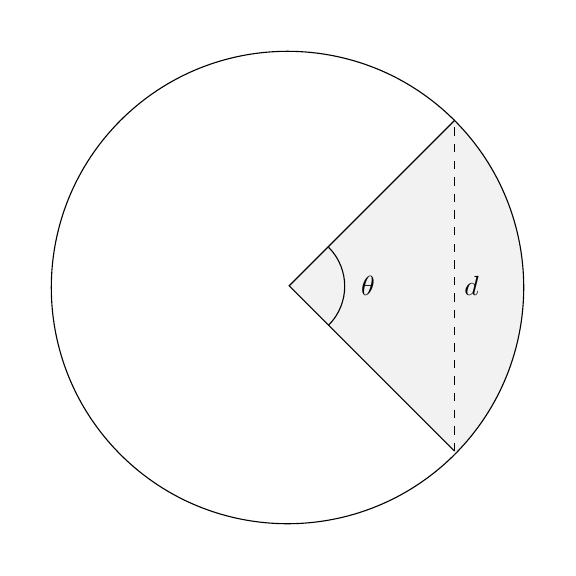
\begin{tikzpicture}
%\draw node[shape=circle, minimum size=6cm, draw]{};
\draw[fill=gray!10] (2.1,-2.1)-- (0,0)--(2.1,2.1) arc(45:-45:3cm);
\draw (2.1,2.1) arc(45:315:3cm);
\draw (.5,-.5) arc(-45:45:.7cm) ;
\draw[dashed] (2.1,-2.1)--(2.1,2.1) node[right, midway]{$d$};
\draw (1,0) node{$\theta$};
\end{tikzpicture}\end{center}

\begin{enumerate}[(a)]
\item
Suppose the angle of the sector is $\theta$. What is the area of the sector?
\item Unfortunately, you don't have a protractor, only a ruler. So, you measure the chord made by the sector (marked $d$ in the diagram above). What is $\theta$ in terms of $d$?
\item Suppose you measured $d=0.7$, but actually $d=0.68$. Estimate the absolute error in your calculation of the area removed.
\end{enumerate}
\end{question}
\begin{hint}
For part (b), cut the triangle (with angle $\theta$ and side $d$) into two right triangles.
\end{hint}
\begin{answer}
(a) $\dfrac{9}{2}\theta$\qquad
(b) $\theta = 2\arcsin\left(\dfrac{d}{6}\right)$\qquad
(c) $\dfrac{9}{\sqrt{36-0.68^2}}\cdot0.02\approx 0.03$
\end{answer}
\begin{solution}
(a) The area removed represents a proportion of $\dfrac{\theta}{2\pi}$ of the entire circle, whose area is $\pi(3^2)=9\pi$. So, the area of the sector removed is
\[\dfrac{\theta}{2\pi} \cdot9\pi = \dfrac{9}{2}\theta\]

(b)
To find $\theta$ from $d$, we cut our triangle (with angle $\theta$ opposite side of length $d$) into two equivalent right triangles, as shown below.
\begin{center}\begin{tikzpicture}
\draw (2.1,-2.1)-- (0,0)--(2.1,2.1) ;
\draw[thick, double] (.5,-.5) arc(-45:45:.7cm) ;
\draw (2.1,-2.1)--(2.1,2.1) node[right, midway]{$d$};
\draw (1,0) node{$\theta$};
\draw (1,1) node[above]{$3$};
\draw[ultra thick, red, ->] (3,0)--(5,0);
\draw (8.1,-2.1)-- (6,0)--(8.1,2.1) ;
\draw (8.1,-2.1)--(8.1,2.1);
\draw (7,1) node[above]{$3$};
\draw[dashed] (6,0)--(8.1,0);
\draw[decorate, decoration={brace, amplitude=10pt, mirror}] (8.25,0)--(8.25,2.1) node[midway, xshift=.75cm]{$\dfrac{d}{2}$};

\draw[thick, double] (6.7,0) arc(0:45:.7cm);
\draw (6.95,.4) node{$\frac{\theta}{2}$} ;
\end{tikzpicture}\end{center}

Using the information that the radius of the circle (also the hypotenuse of the right triangle) is 3,
\begin{align*}
\sin\left(\frac{\theta}{2}\right)&=\frac{\frac{d}{2}}{3}=\frac{d}{6}
\intertext{Since the question tells us the sector is no more than a quarter of the circle, we know $0 \leq \theta \leq \dfrac{\pi}{2}$, so $0 \leq \dfrac{\theta}{2} \leq \dfrac{\pi}{4}$. This puts $\dfrac{\theta}{2}$ well within the range of arcsine.}
\theta&=2\arcsin\left(\frac{d}{6}\right)
\end{align*}

(c) First, let's
get an expression for the area of the sector in terms of $d$.
\begin{align*}
A&=\frac{9}{2}\theta = \frac{9}{2}\left(2\arcsin\left(\frac{d}{6}\right)\right)
\\&=9\arcsin\left(\frac{d}{6}\right)
\intertext{Differentiating,}
A'(d)&=\frac{9}{\sqrt{1-\left(\frac{d}{6}\right)^2}}\cdot\frac{1}{6}\\
&=\frac{9}{\sqrt{36-d^2}}
\intertext{Let $\Delta A$ is the error in $A$ corresponding to an error of $\Delta d$ in $d$.
Since we measured $d$ to be 0.7 instead of $0.68$, in the linear approximation we take $\Delta d = 0.02$ and $d_0=0.68$.}
\Delta A &\approx A'(d_0)\cdot\Delta d\\
&=A'\left(0.68\right)\cdot 0.02\\
&=\frac{9}{\sqrt{36-0.68^2}}\cdot0.02\\
&\approx 0.03
\end{align*}
So, the error in $A$ is about 0.03.
\end{solution}




\begin{question}
A conical tank, standing on its pointy end, has height 2 metres and radius 0.5 metres.
Estimate change in volume of the water in the tank associated to a change in the height of the water from 50 cm to 45 cm.
\begin{center}\begin{tikzpicture}
\draw(0,3) node[shape=ellipse, minimum height=1.25cm, minimum width=3cm, draw]{};
\draw (1.5,3)--(0,-1)--(-1.5,3);
\draw (0,3)--(1.5,3) node[above, midway]{$0.5$};
\draw[decorate, decoration={brace, amplitude=10pt}] (-2,-1)--(-2,3) node[midway, xshift=-.75cm]{2};
 \draw[fill=blue!20] (-.375,0) arc
  (180:360:.375cm and .1875cm)--(0,-1)--cycle;
\end{tikzpicture}\end{center}
\end{question}
\begin{hint}
The volume of a cone of height $h$ and radius $r$ is
        $\frac{1}{3}\pi r^2 h$.
\end{hint}
\begin{answer}
We estimate that the volume decreased by about $0.00245$ cubic metres, or about
2450 cubic centimetres.
\end{answer}
\begin{solution}
Suppose we have a function $V(h)$ that gives the volume of water in the tank as a function of its height. \\
Let $h_0=0.5$ metres, $\Delta h = -0.05$, and $\Delta V  = V(h_0+\Delta h)-V(h_0)=V(0.45)-V(0.5)$. Then, by the linear approximation,
\[
\Delta V \approx V'(0.5)\cdot \Delta h = -0.05V'(0.5)\]
\textcolor{red}{In order to solve the problem, we will find a function $V(h)$ giving the volume of water in terms of the height, then find $V'(0.5)$,  and finally approximate that the change in the volume of the water is $\Delta V \approx -0.05V'(0.5)$.}

The water in the tank forms a cone. The volume of a cone of height $h$ and radius $r$ is
\[
V=\frac{1}{3}\pi r^2 h\]
We need to get rid of the variable $r$. We can do this using similar triangles. The diagram below shows the side view of the tank and the water.
\begin{center}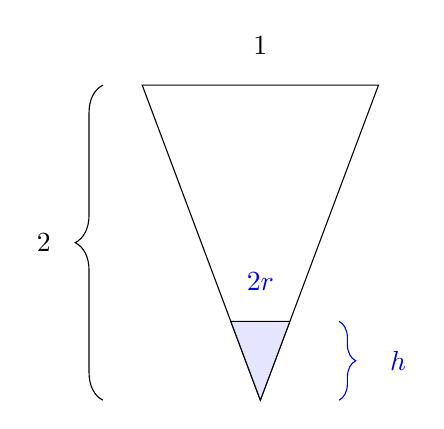
\begin{tikzpicture}
\draw (-1.5,3)--(0,-1)--(1.5,3)--cycle;
\draw (0,3.5) node{1};
\draw[fill=blue!10] (-.375,0)--(0,-1)--(.375,0)--cycle;
\draw[blue] (0,.5) node{$2r$};
\draw[decorate, decoration={brace, amplitude=10pt}] (-2,-1)--(-2,3) node[midway, xshift=-.75cm]{2};
\draw[blue,decorate, decoration={brace, amplitude=6pt, mirror}] (1,-1)--(1,0) node[midway, xshift=.75cm]{$h$};
\end{tikzpicture}\end{center}
The side view of the tank forms a triangle that is similar to the triangle formed by the side view of the water, so
\begin{align*}
\frac{1}{2}&=\frac{2r}{h}\\
r&=\frac{h}{4}
\intertext{Using this, we find our equation for the volume of the water in terms of $h$.}
V(h)&=\frac{1}{3}\pi r^2 h = \frac{\pi}{3}\left(\frac{h}{4}\right)^2h=\frac{\pi h^3}{48}
\intertext{Differentiating,}
V'(h)&=\frac{\pi h^2}{16}\\
V'(0.5)&=\frac{0.25\pi}{16}=\frac{\pi}{64}
\intertext{Finally, using the approximation $\Delta V \approx -0.05V'(0.5)$,}
\Delta V &\approx \frac{-0.05\pi}{64}=-\frac{\pi}{1280}\approx -0.00245 ~\mathrm{m}^3
\end{align*}
We estimate that the volume decreased by about $0.00245$ cubic metres, or about
2450 cubic centimetres.
\end{solution}



%%%%%%%%%%%%%%%%%%
\subsection*{\Application}
%%%%%%%%%%%%%%%%%%



\begin{question}
A sample begins with precisely 1 $\mu$g of a radioactive isotope, and after 3 years is measured to have 0.9 $\mu$g remaining. If this measurement is correct to within 0.05 $\mu$g, estimate the corresponding accuracy of the half-life calculated using it.
\end{question}
\begin{hint}
Remember that the amount of the isotope present at time $t$ is $Q(t)=Q(0)e^{-kt}$ for some constant $k$. The measured quantity after 3 years will allow you to replace $k$ in the equation, then solving $Q(t)=\frac{1}{2}Q(0)$ for $t$ will give you the half-life of the isotope.
\end{hint}
\begin{answer} Correct to within about 10.4 years (or about 53\%)
\end{answer}
\begin{solution}
Let $q$ be the measured amount of the isotope remaining after 3 years. Let $h(q)$ be the half-life of the isotope that we calculate using $q$.
We measured $q=0.9$, but we want to know what the change in $h$ is if $q$ moves by 0.05. So, let $\Delta q= \pm 0.05$, and let $\Delta h$ be the corresponding change in $h$.
The linear approximation tells us
\begin{align*}\Delta h& \approx h'(0.9)\Delta q
\intertext{So,}
\left|\Delta h\right|&\approx\left| h'(0.9)\right|\left|\Delta q\right|= h'(0.9)\cdot 0.05
\end{align*}
\textcolor{red}{This suggests a plan for solving the problem. We will find the equation $h(q)$ giving the calculated half-life of the isotope based on the measurement $q$. Then, we will find $h'(0.9)$. Finally, the equation $\left|\Delta h\right|=h'(0.9)\cdot0.05$ will tell us the change in $h$ that corresponds with a change of 0.05 in our measurement.}

Let us find the half-life of the isotope, if after three years $q$ $\mu$g is remaining. The amount of the isotope present after $t$ years is given by
\begin{align*}
Q(t)&=Q(0)e^{-kt}
\intertext{for some constant $k$. Let's take $t=0$ to be the time when precisely one $\mu$g was present. Then}
Q(t)&=e^{-kt}
\intertext{After three years, $q$ is the amount of the isotope remaining, so}
q&=e^{-k\cdot 3}\\
q^{\frac{1}{3}}&=e^{-k}\\
Q(t)&=\left(e^{-k}\right)^t=q^{\frac{t}{3}}
\intertext{The half-life is the value of $t$ for which $Q(t)=\frac{1}{2}Q(0)=\frac{1}{2}$.}
\frac{1}{2}&=Q(t)=q^{\frac{t}{3}}\\
\log\left(\frac{1}{2}\right)&=\log\left(q^{\frac{t}{3}}\right)\\
-\log 2 &=\frac{t}{3}\log q\\
t&=\frac{-3\log 2}{\log q}
\end{align*}
So, we calculate the half-life to be $\dfrac{-3\log 2}{\log q}$. This gives us our first goal: a function $h(q)$ that tells us the calculated half-life of the element.
\begin{align*}h(q)&=\dfrac{-3\log2}{\log q}
\intertext{Following our plan, we find $h'(0.9)$.}
h'(q)&=\diff{}{q}\left\{\dfrac{-3\log2}{\log q}\right\}\\
&=-3\log 2\cdot\diff{}{q}\left\{\left(\log q\right)^{-1}\right\}\\
&=-3\log 2\cdot(-1)\left(\log q\right)^{-2}\cdot\frac{1}{q}\\
&=\frac{3\log 2}{q\log^2q}\\
h'(0.9)&=\frac{3\log2}{0.9\log^2(0.9)}\approx 208
\intertext{Finally, as outlined in our plan, }
\left|\Delta h\right|&=h'(0.9)\cdot0.05\\
&=\frac{3\log2}{18\log^2(0.9)}\approx 10.4
\end{align*}
If our measurement changes by $\pm 0.05$ $\mu$g, then we estimate our calculated half-life changes by about $\pm$10.4 years. Since our measurement is accurate to within $0.05$ $\mu$g, that means we estimate
our calculated half-life to be accurate to within about 10.4 years.

Remark: since $h(0.9)=\dfrac{-3\log 2}{\log 0.9} \approx 19.7$, an absolute error of 10.4 years corresponds to a percentage error of $100\dfrac{10.4}{19.7}\approx 53\%$. The question did not specify absolute or percentage error. Since both make sense, you can use either one.
\end{solution}
